\subsection{Tính Chất Nâng Cao}
% -----------------------------------------------------------------------------

Bốn kết quả lý thuyết sau giải thích tại sao tuyến tính trong tham số tạo ra sự đảm bảo mạnh mẽ hơn nhiều so với những gì các công cụ chẩn đoán thực hành gợi ý.

% - - - - - - - - - - - - - - - - - - - - - - - - - - - - - - - - - - - - - -
\subsubsection{Chiếu Trực Giao Lên Không Gian Dự Báo}

Hình ảnh thông thường của hồi quy là một mặt phẳng qua dữ liệu ba chiều. Bức tranh sâu hơn sống trong không gian $n$ chiều. Mỗi quan sát $Y$ là một điểm trong $\mathbb{R}^n$. Các cột của ma trận thiết kế $X$ trương ra một không gian con thấp chiều hơn---\textbf{không gian dự báo} (column space của $X$). Vì mô hình tuyến tính, tìm $\hat{\beta}$ tương đương với tìm điểm trong không gian dự báo \textit{gần nhất} với $Y$:
\[
  \hat{Y} = X(X^\top X)^{-1}X^\top Y = P_X Y
\]
trong đó $P_X$ là ma trận chiếu trực giao lên $\mathrm{Col}(X)$.

Vector sai số $e = Y - \hat{Y}$ trực giao với mọi cột của $X$---đây không phải xấp xỉ, mà là hệ quả hình học chính xác của OLS. Hệ phương trình chuẩn $X^\top e = 0$ chính là phát biểu đại số của điều kiện trực giao này. Hầu hết lý thuyết mô hình tuyến tính---từ định lý Gauss-Markov đến hình học kiểm định $F$---đều bắt nguồn trực tiếp từ cấu trúc chiếu trực giao này.

\begin{figure}[H]
  \centering
  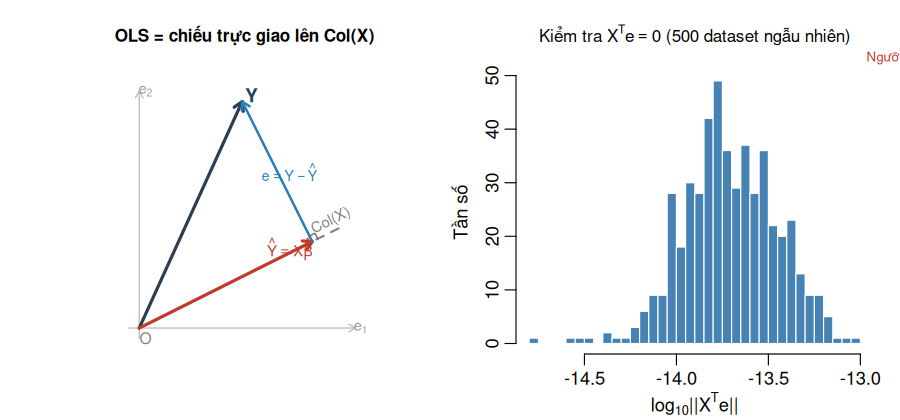
\includegraphics[width=\textwidth]{./figures/fig10_projection.png}
  \caption{\textbf{Trái:} Sơ đồ hình học của OLS trong $\mathbb{R}^n$.
  $Y$ là điểm quan sát, $\hat{Y} = P_X Y$ là hình chiếu vuông góc lên $\mathrm{Col}(X)$, và $e = Y - \hat{Y}$ là vector sai số vuông góc với không gian dự báo.
  \textbf{Phải:} Xác minh số trên 500 dataset ngẫu nhiên ($n = 40$, $p = 3$).
  Giá trị $\log_{10}\|X^\top e\|$ luôn ở mức sai số máy tính ($\approx 10^{-12}$), xác nhận $X^\top e = 0$ là đẳng thức chính xác, không phải xấp xỉ.}
  \label{fig:projection}
\end{figure}

% - - - - - - - - - - - - - - - - - - - - - - - - - - - - - - - - - - - - - -
\subsubsection{Phân Phối Chuẩn Đa Biến Đảm Bảo Tuyến Tính}

Tuyến tính thường là giả định làm việc về thế giới. Một trường hợp nó được đảm bảo bởi toán học: nếu biến phản hồi $Y$ và các biến dự báo $X_1, \ldots, X_p$ cùng tuân theo \textbf{phân phối chuẩn đa biến}, thì từ tính chất của phân phối chuẩn đa biến, phân phối có điều kiện là:
\[
  Y \mid X \sim \mathcal{N}(X\beta,\ \sigma^2)
\]

Kỳ vọng có điều kiện $E[Y \mid X] = X\beta$ là tuyến tính trong $X$, và phương sai có điều kiện $\sigma^2$ là hằng số---cả hai đều bắt nguồn từ cấu trúc ma trận hiệp phương sai của phân phối chuẩn đa biến, không từ bất kỳ giả định ngoại sinh nào. Nếu dữ liệu có thể xuất từ phân phối chuẩn đa biến (kiểm tra bằng Q-Q plot đa biến hoặc kiểm định Mardia), không cần giả định tuyến tính riêng biệt.

% - - - - - - - - - - - - - - - - - - - - - - - - - - - - - - - - - - - - - -
\subsubsection{Định Lý Li-Duan: Bền Vững Trước Phi Tuyến Ẩn}

Giả sử quan hệ thực là phi tuyến nhưng có dạng chỉ số đơn:
\[
  E[Y \mid X] = g(\beta^\top x)
\]
trong đó $g$ là hàm \textit{hoàn toàn ẩn}. Bình thường điều này dường như làm mất hiệu lực OLS hoàn toàn. \textbf{Định lý Li-Duan (1989)} cho thấy điều ngược lại: nếu các biến dự báo $X$ tuân theo phân phối đối xứng elip (bao gồm phân phối chuẩn đa biến), thì OLS vẫn ước lượng $\beta$ \textbf{nhất quán đến một hằng số tỷ lệ}:
\[
  \hat{\beta}_{\text{OLS}} \xrightarrow{p} c \cdot \beta, \quad c \neq 0
\]

Nói cách khác: ngay cả khi dạng hàm thực sự bị ẩn và phi tuyến, mô hình tuyến tính khớp một cách mù quáng vẫn phục hồi đúng \textit{hướng} và \textit{tầm quan trọng tương đối} của các biến dự báo. Độ lớn bị chia tỷ lệ, nhưng thứ hạng và dấu của tác động được bảo toàn.

\begin{figure}[H]
  \centering
  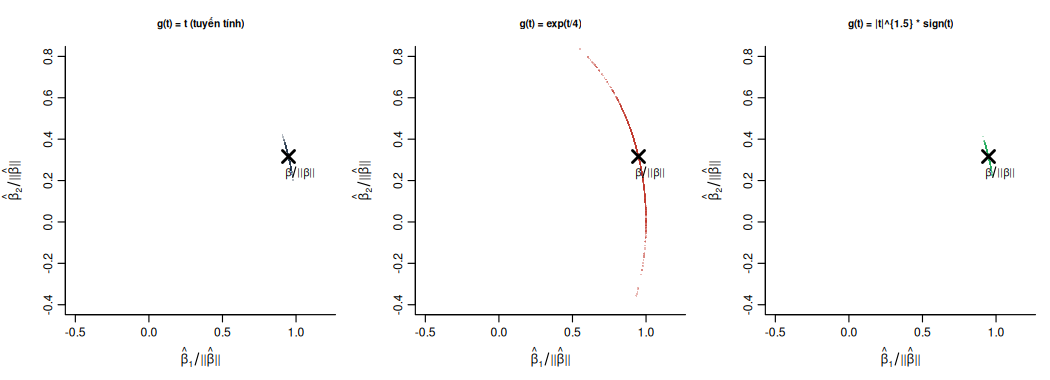
\includegraphics[width=\textwidth]{./figures/fig11_liduan.png}
  \caption{Mô phỏng định lý Li-Duan ($n = 60$, $B = 800$ lần lặp).
  Mô hình thực: $Y = g(\beta^\top X) + \varepsilon$ với $\beta = (3, 1)^\top$ và $X \sim \mathcal{N}(0, I)$.
  Mỗi điểm là hướng ước lượng $\hat{\beta} / \|\hat{\beta}\|$ từ một lần lặp.
  Dấu ``$\times$'' là hướng thực $\beta / \|\beta\|$.
  Ba hàm $g$ khác nhau (tuyến tính, mũ, lũy thừa có dấu) đều cho đám mây điểm tập trung tại cùng một hướng thực---OLS phục hồi đúng hướng bất kể dạng hàm.}
  \label{fig:liduan}
\end{figure}

% - - - - - - - - - - - - - - - - - - - - - - - - - - - - - - - - - - - - - -
\subsubsection{Bất Biến Trước Biến Đổi Tuyến Tính Toàn Hạng}

Vì dự báo $\hat{Y}$ là chiếu trực giao của $Y$ lên $\mathrm{Col}(X)$, và $\mathrm{Col}(X)$ không thay đổi khi nhân $X$ với bất kỳ ma trận toàn hạng nào, ta có:

\textbf{Định lý:} Với mọi ma trận toàn hạng $A$ ($k \times k$), mô hình $Y \sim XA$ cho ra các giá trị khớp $\hat{Y}$, phần dư $e$, và phương sai sai số $s^2$ \textit{hoàn toàn giống} mô hình $Y \sim X$.

\textbf{Hệ quả thực tiễn:} Centering, scaling, và orthogonalization là các bước tiền xử lý \textit{an toàn}---chúng thay đổi tham số hóa nhưng không bao giờ thay đổi dự báo hay $R^2$.

\textbf{Giải thích đa cộng tuyến:} Đa cộng tuyến làm các hệ số riêng lẻ $\hat{\beta}_j$ không ổn định (vì $\hat{\beta}$ không bất biến với biến đổi tuyến tính), nhưng hoàn toàn không ảnh hưởng đến giá trị khớp $\hat{Y}$ hay khả năng dự báo tổng thể (vì $\hat{Y}$ bất biến).

\begin{lstlisting}[style=Rstyle]
# Xac minh: standardize X khong lam thay doi y_hat va R2
fit_raw  <- lm(mpg ~ hp + wt + disp, data = mtcars)
fit_std  <- lm(mpg ~ scale(hp) + scale(wt) + scale(disp), data = mtcars)

max(abs(fitted(fit_raw) - fitted(fit_std)))  # < 1e-12
summary(fit_raw)$r.squared - summary(fit_std)$r.squared  # = 0
\end{lstlisting}

\begin{lstlisting}[style=output]
[1] 1.065814e-13
[1] 0
\end{lstlisting}

